Kryosféra je termín zastřešující veškerou vodu v pevném skupenství (ledu), která se nachází na zemském povrchu. Komponenty kryosféry a jejich délka trvání je znázorněna na obr. \ref{fig:komponentykryosfery}. Jednou z nejdůležitějších komponent jsou ledovce. 
\begin{figure*}
	\centering
	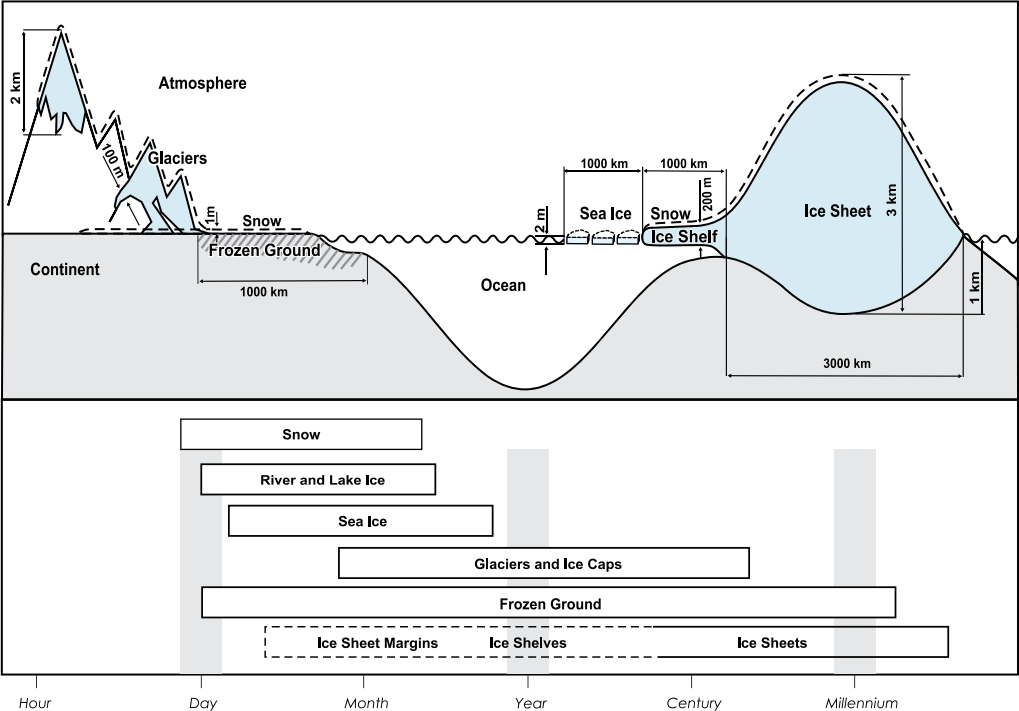
\includegraphics[width=1\linewidth]{obrazky/glac/komponenty_kryosfery}
	\caption{Komponenty kryosféry a jejich časové škály (převzato z \textcite{lemkeObservationsChangesSnow2007})}
	\label{fig:komponentykryosfery}
\end{figure*}

\section{Ledovce}
\emph{Ledovce} jsou tekoucí tělesa ledu, která pokrývají zemskou souš. V současné tak činí z cca $10 \%$ \parencite{cuffeyPhysicsGlaciers2010}), v dobách maximálního zalednění to byl ale zhruba trojnásobek. Vlivem klimatické změny ale dochází k rychlým změnám v celkovém objemu a rozloze ledovců. V období 2000--2019 činila ztráta hmoty ledovců okolo \SI{270}{\giga\tonne\per\rok} \parencite{hugonnetAcceleratedGlobalGlacier2021}.

\subsection{Vznik ledovců a bilance hmoty}
Čerstvě napadaný sníh má velice nízkou hustotu (tab. \ref{tab:snih_led}). Postupnou kompakcí vlivem tlaku sněhové hmoty v nadloží a rekrystalizací se jeho hustota zvyšuje a mění se ve \emph{firn}. Další kompakcí, zcelováním jednotlivých ledových krystalů do jednolité hmoty se firn mění v \emph{ledovcový led} jehož hustota se pohybuje mezi \SIrange{830}{923}{\kilogram\per\cubic\metre} (tab. \ref{tab:snih_led}; \textcite{cuffeyPhysicsGlaciers2010}). 

\begin{table}[h]
	\centering
	\caption{Typická hustota sněhu, firnu a ledovcového ledu v \si{\kilogram\per\cubic\metre}(upraveno podle \textcite{cuffeyPhysicsGlaciers2010})}
	\begin{tabularx}{0.9\linewidth}{@{}XS@{}}
		\toprule
		Čerstvě napadaný sníh	 & \numrange{50}{70}  \\
		Zvlhlý čerstvý sníh		 & \numrange{100}{200}\\
		Uleželý sníh        	 & \numrange{200}{300}\\
		Větrem utužený sníh      & \numrange{350}{400}\\
		Firn                     & \numrange{400}{830}\\
		Velice mokrý sníh a firn & \numrange{700}{800}\\
		Ledovcový led            & \numrange{830}{923}\\ \bottomrule
	\end{tabularx}
	\label{tab:snih_led}
\end{table}

Ledovce mění svůj objem v závislosti na přísunu hmoty (ledu) -- \emph{akumulaci}, a jeho úbytku neboli \emph{ablaci}. Přírůstky ledu jsou způsobené zejména sněhovými srážkami, které dopadají přímo na ledovec nebo jsou na něj dopraveny pomocí lavin či převáty větrem z okolí. Úbytek hmoty je způsoben táním ledu a následným odtokem tavných vod, odlamování ker (tzv. telení), větrnou erozí, ale i sublimací ledu (přímou přeměnou ledu ve vodní páru). 

Na ledovci rozlišujeme z hlediska bilance dvě záklaní zóny: akumulační a ablační (Obr \ref{fig:ledovecmassbalance}). Do \emph{akumulační zóny} spadá ta část ledovce, která má pozitivní bilanci (přírůstky hmoty). \emph{Ablační zóna} má zápornou bilanci, dochází zde k úbytku hmoty. Hranicí mezi akumulační a ablační zónou je tzv. \emph{čára rovnováhy} (\textit{equilibrium line altitude}). Pokud je celková bilance ledovce záporná, ledovec se zmenšuje a naopak. Bilance hmoty v ledovci se zpravidla určuje pro období mezi dvěma okamžiky, kdy ablace dosáhla svého maxima (konec léta 1 -- konec léta 2).

%TODO ukázka měření pomocí ablační tyče
%\begin{myboxgreenwide}{Jak se měří bilance hmoty v ledovci?}
%hsfgoisdiofgjoisdjf sdfoig jdsoifjg osdijf sdofijg osdifj odsj
%\end{myboxgreenwide}

\begin{figure*}
	\centering
	\includegraphics[width=\linewidth]{obrazky/glac/ledovec_mass_balance}
	\caption{Ablační a akumulační zóna na idealizovaném ledovci a jeho bilance hmoty (upraveno podle \textcite{summerfieldGlobalGeomorphologyIntroduction1999})}
	\label{fig:ledovecmassbalance}
\end{figure*}

\subsection{Typy ledovců}
Základní klasifikace ledovců na ty, které nejsou limitované reliéfem (např. Grónský ledový příkrov) a ty které jsou nějak omezené reliéfem jako je v případě údolních ledovců v Alpách.

\subsubsection{Ledové příkrovy, čapky a šelfové ledovce}
\emph{Ledový příkrov} (\enquote{ice sheet}) neboli také \emph{ledový štít} či \emph{kontinentální ledovec} je nejrozsáhlejší ledovcové těleso. Jejich plocha musí přesahovat \SI{50000}{\square\kilo\metre}. V současné době se ledové příkrovy nacházejí jen v Grónsku a Antarktidě. \emph{Ledová čapka} (\enquote{ice cap}) je prakticky malou verzí ledového příkrovu. 
Jedná se o obrovské masy ledu, které zcela překrývají topografii. Ledový příkrov se skládá ze dvou základních částí. \emph{Ledové dómy} jsou konvexní formy, ledové vyvýšeniny z nichž se led radiálně roztéká. 
\emph{Ledové proudy} jsou části ledového příkrovu nebo ledové čapky, kde se led pohybuje významně rychleji než v okolních částech. Ve srovnání s celým ledovým příkrovem se jedná o relativně úzké oblasti, ale prostřednictvím těchto proudů je transportována převážná část ledové hmoty příkrovů. 

\emph{Šelfový ledovec} je část ledovce, která plave na hladině oceánu či moře. 

\begin{figure*}[h]
	\centering
	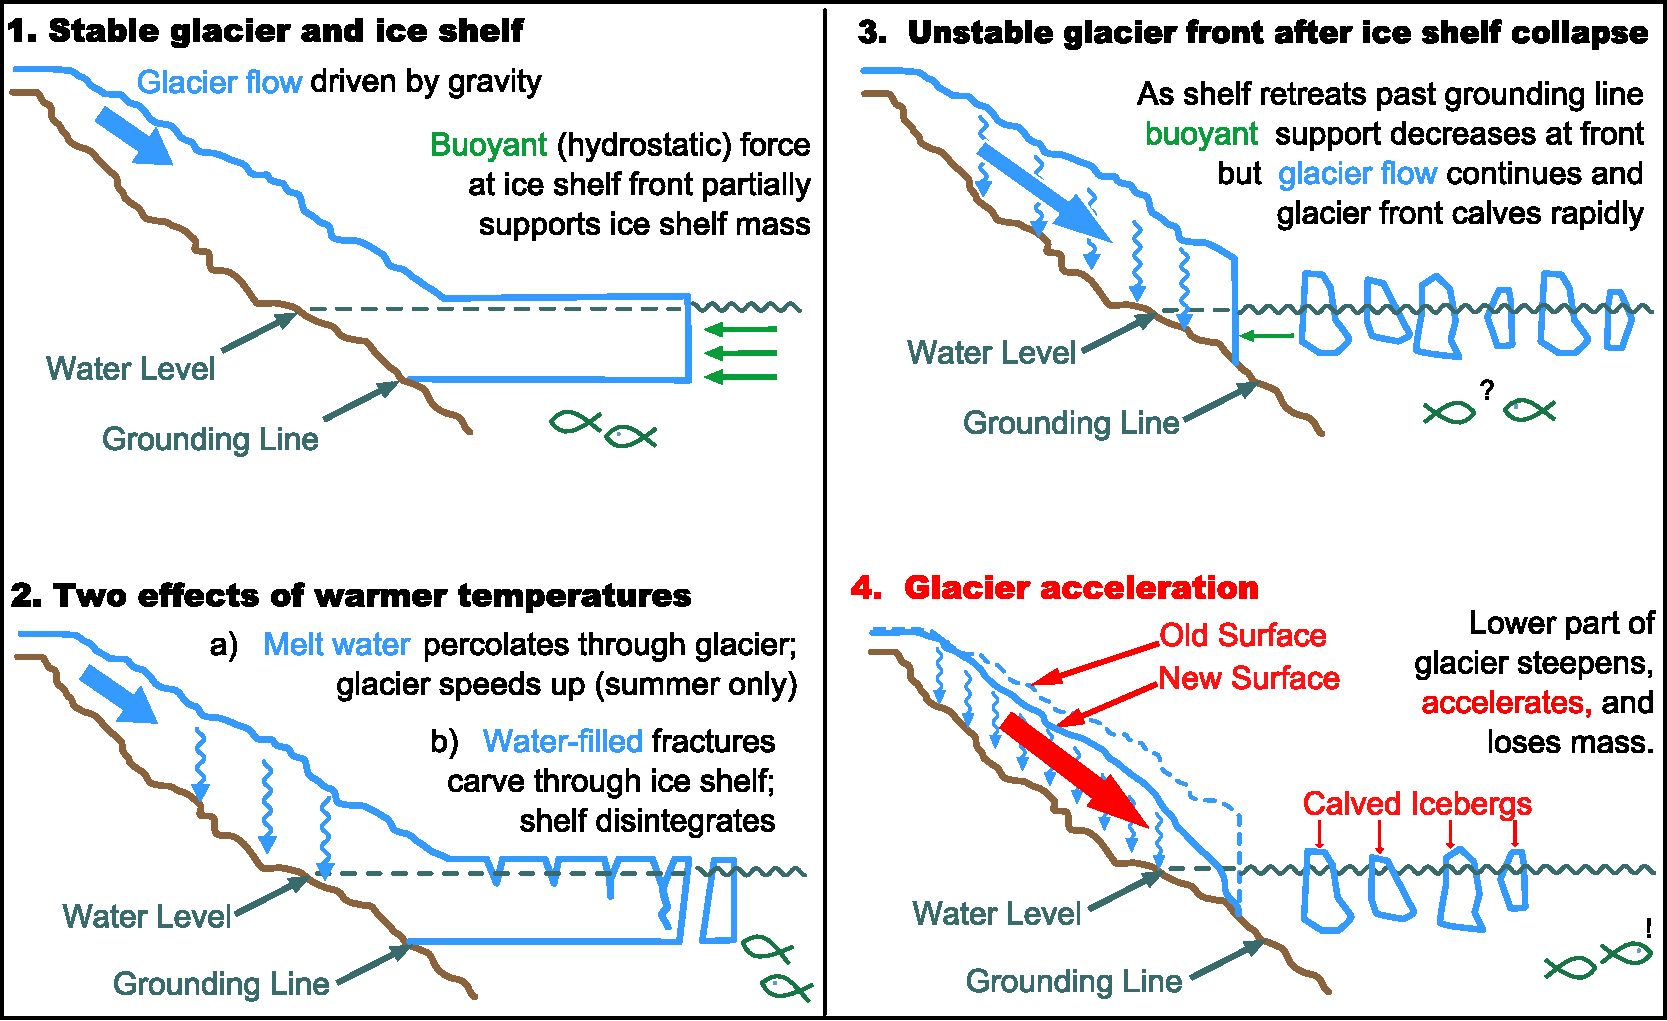
\includegraphics[width=1\linewidth]{obrazky/glac/iceshelf}
	\caption{Šelfový ledovec a jeho interakce s okolním prostředím. V případě, že šelfový ledovec je stabilní, podpírá a zpomaluje celkový pohyb ledovce. Zvýšené teploty způsobují dvě věci: 1. rychlejší tání ledovce, voda se dostává na bázi, snižuje tření ledovce a urychluje jeho pohyb; 2. vznik a rozšiřování puklin vyplněných vodou na šelfu urychluje jeho rozpad. V případě rozpadu ledovcového šelfu ledovec ztrácí oporu a rychlost jeho pohybu se zvyšuje a tedy i rychleji ztrácí hmotu (autoři: Ted Scambos and Michon Scott, National Snow and Ice Data Center, upraveno: Sagredo, volné dílo, via Wikimedia Commons)}
	\label{fig:iceshelf}
\end{figure*}

\subsubsection{Ledovce limitované topografií}
Mezi ledovce, které jsou ovlivněné či řízené reliéfem řadíme \emph{Ledovcová pole} a hlavně \emph{horské ledovce} (\enquote{mountain glaciers}).

\emph{Ledovcová pole} (\enquote{ice fields}) připomínají ledové čapky, avšak nemají kopulovitou topografii, takže tok ledu je řízen hlavně reliéfem v podloží.

Velkou skupinu tvoří \emph{horské ledovce}. \emph{Svahové ledovce} vznikají v mělkých depresích či strukturních stupních na příkrých svazích. \emph{Karový ledovec} (\enquote{cirque (corrie) glacier}) je relativně malý ledovec, který vyplňuje \emph{kar}. Kar je oválná deprese, která je otevřená jedním směrem a byla vytvořená erozivní činností ledovce. Když karový ledovec přeteče přes hranu karu do údolí, stává se z něj \emph{údolní ledovec} (někdy se dodává alpského typu, angl. \enquote{valley glacier}). Ledovce vytékající až do podhůří, kde se mohou spojovat do jednoho velkého lemu se nazývají \emph{úpatní} nebo \emph{piedmontní} ledovce (\enquote{piedmont glaciers}).
%TODO obrázky ledovců


\subsubsection{Typy ledovců podle teploty báze}
%TODO Báze
Velice důležitým faktorem, který ovlivňuje pohyb ledovce a jeho schopnost modelovat své podloží, je teplota báze ledovce (rozhraní ledovec--podloží). \emph{Ledovec s chladnou bází} má na kontaktu s podložím takovou teplotu, při které led netaje. Ledovec je přimrzlý k podloží. Důsledkem toho takový ledovec nemodeluje své podloží. \emph{Ledovec s teplou bází} je naopak na kontaktu roztáté. Nachází se tam množství tavné vody. Ledovce s teplou bází intenzivně modelují své podloží. \emph{Polytermální ledovce} jsou na pomezí předešlých dvou typů. Jedná se většinou o rozsáhlejší ledovce, kde se střídají oblasti s chladnou a teplou bází. 

\subsection{Pohyb ledovců}
Působením tíhové síly je v ledovci vyvoláváno smykové napětí, které uvádí ledovce do pohybu. Rozlišujeme dva základní mechanismy. První mechanismus, kterým se pohybují všechny ledovce je vnitřní (plastická) deformace nazývaná ledovcový kríp (\enquote{ice creep}). Druhý mechanismus je \emph{bazální klouzání} (smýkání). Ledovce s teplou bází se dominantně pohybují bazálním smýkáním, vnitřní deformací samotného ledu je realizován jen zlomek celkového pohybu. U ledovců se studenou bází to je naopak. Bazální klouzání je téměř nulové a ledovcová masa se pohybuje vnitřní deformací ledu. 

\begin{figure*}
	\centering
	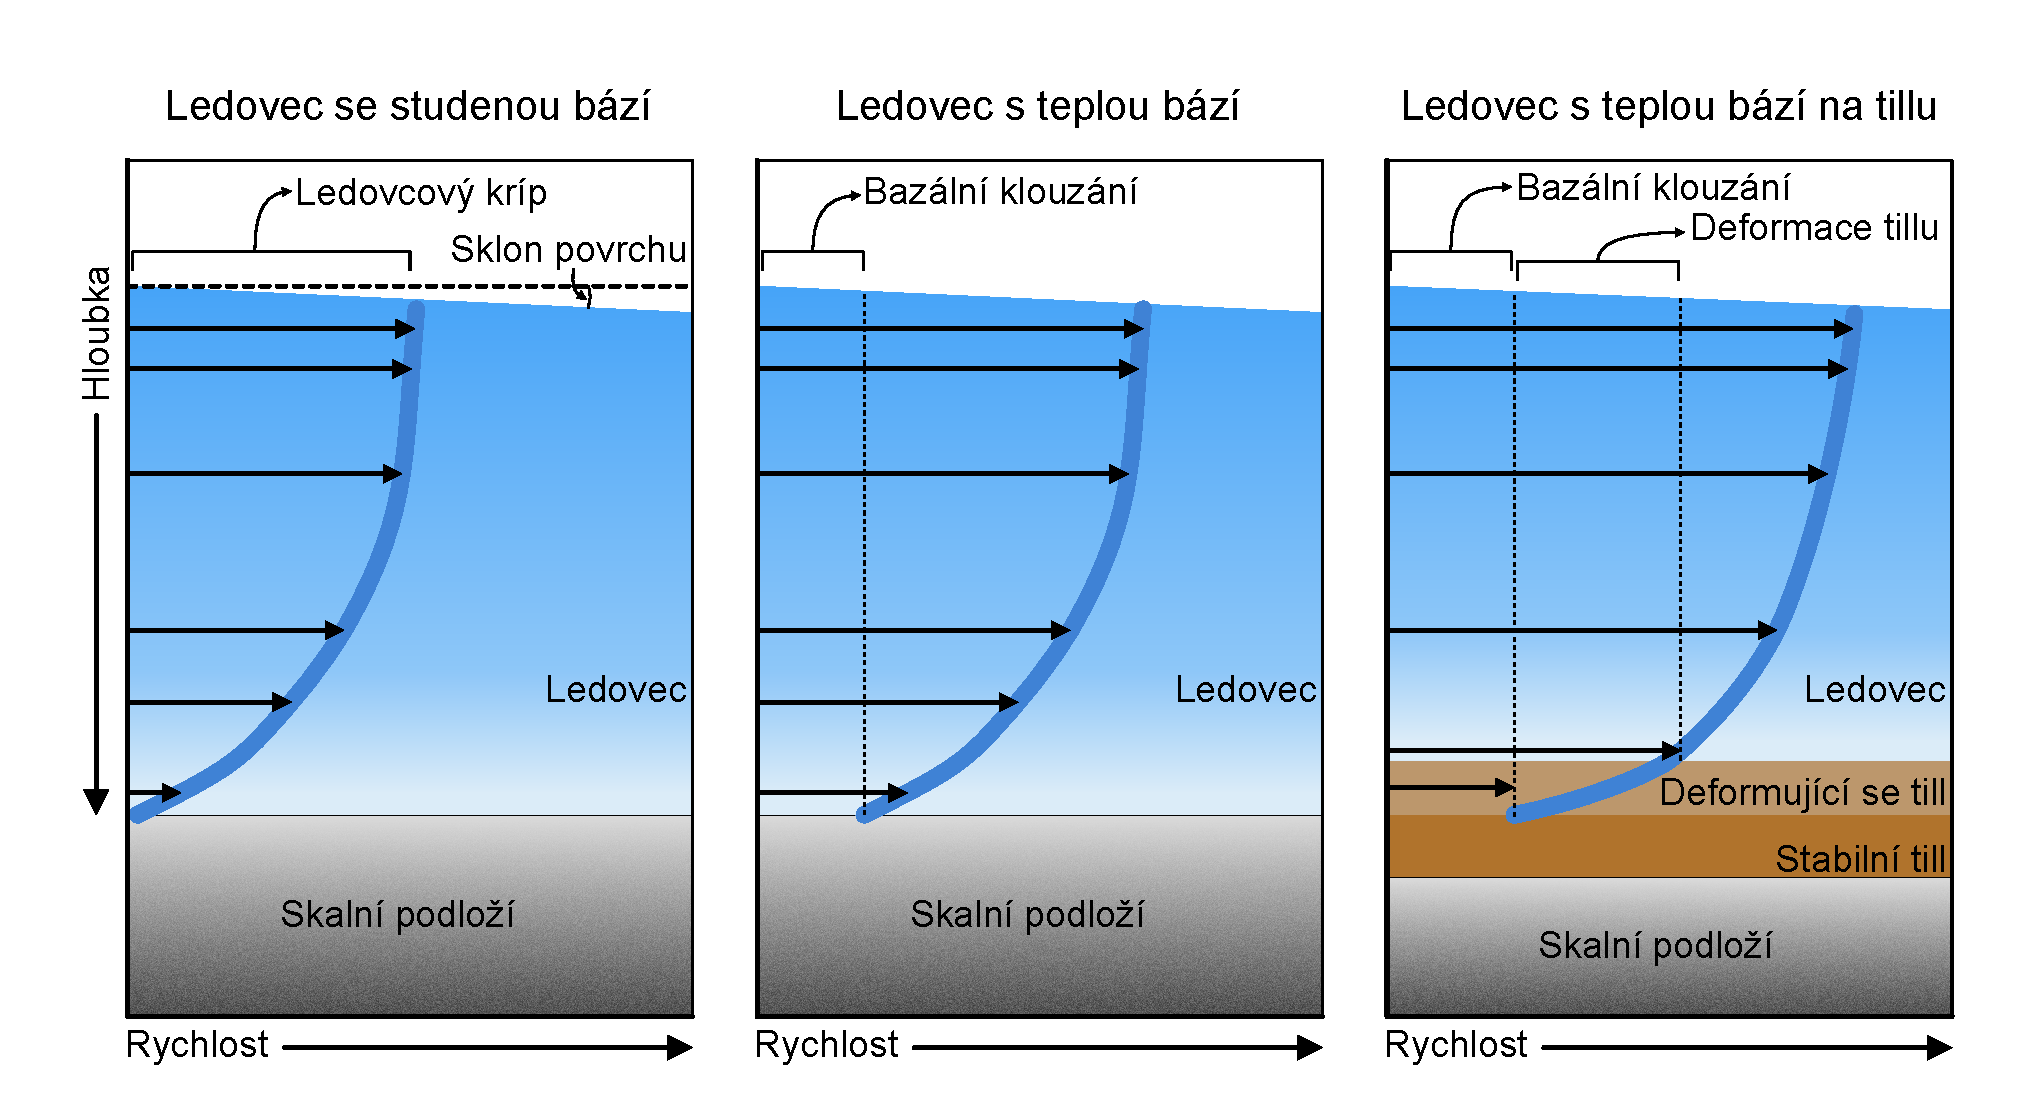
\includegraphics[width=1\linewidth]{obrazky/glac/flow_velocity}
	\caption{Rychlost pohybu ledovce v závislosti na teplotě báze a přítomnosti tillu (Upraveno podle \textcite{biermanKeyConceptsGeomorphology2014})}
	\label{fig:flowvelocity}
\end{figure*}

Rychlost deformace ledu (\enquote{strain rate}, $\dot{\epsilon}$) je dána experimentálně odvozenou Glenovou rovnicí:

\begin{equation}
	\dot{\epsilon} = A\tau^{n}
\end{equation}

\begin{eqexpl}
	\item{$\dot{\epsilon}$} je rychlost deformace
	\item{$A$}je koeficient, který s teplotou roste
	\item{$\tau$}je střižné (smykové) napětí 
	\item{$n$}experimentálně zjištěný exponent, pro led platí, že $n \approx 3$
\end{eqexpl}

Jak je patrné z rovnice (jelikož $n > 1$), tak i malé změny smykového napětí  vedou k velkým změnám v úrovni deformace.

Průměrná rychlost pohybu ledovce je v rozmezí \SIrange{3}{300}{\metre\per\rok}. Rychlost pohybu se mění v prostoru a čase. Největší rychlost pohybu ledovce je na jeho povrchu a směrem dolů klesá (Obr. \ref{fig:flowvelocity}). V podélném profilu se rychlost mění v závislosti na akumulaci a ablaci.

%TODO Morfologie povrchu ledovců
%\section{Morfologie povrchu ledovců}

\section{Glaciální procesy}

\subsection{Erozní činnost ledovců}
Celkem rozlišujeme čtyři mechanismy glaciální eroze. \emph{Deterze} je ohlazování skalního podloží. \emph{Exarace} rýhování skalního podloží. Tímto procesem vznikají striace. Podle striací skalního podloží lze určit směr pohybu ledovce. \emph{Detrakce} je proces odlamování Čtvrtý mechanismus \emph{plucking} je spojený s účinky mrazového zvětrávání a tlaku ledovce. Jedná se o vytrhování kusů horniny z podloží.

\begin{figure}
	\centering
	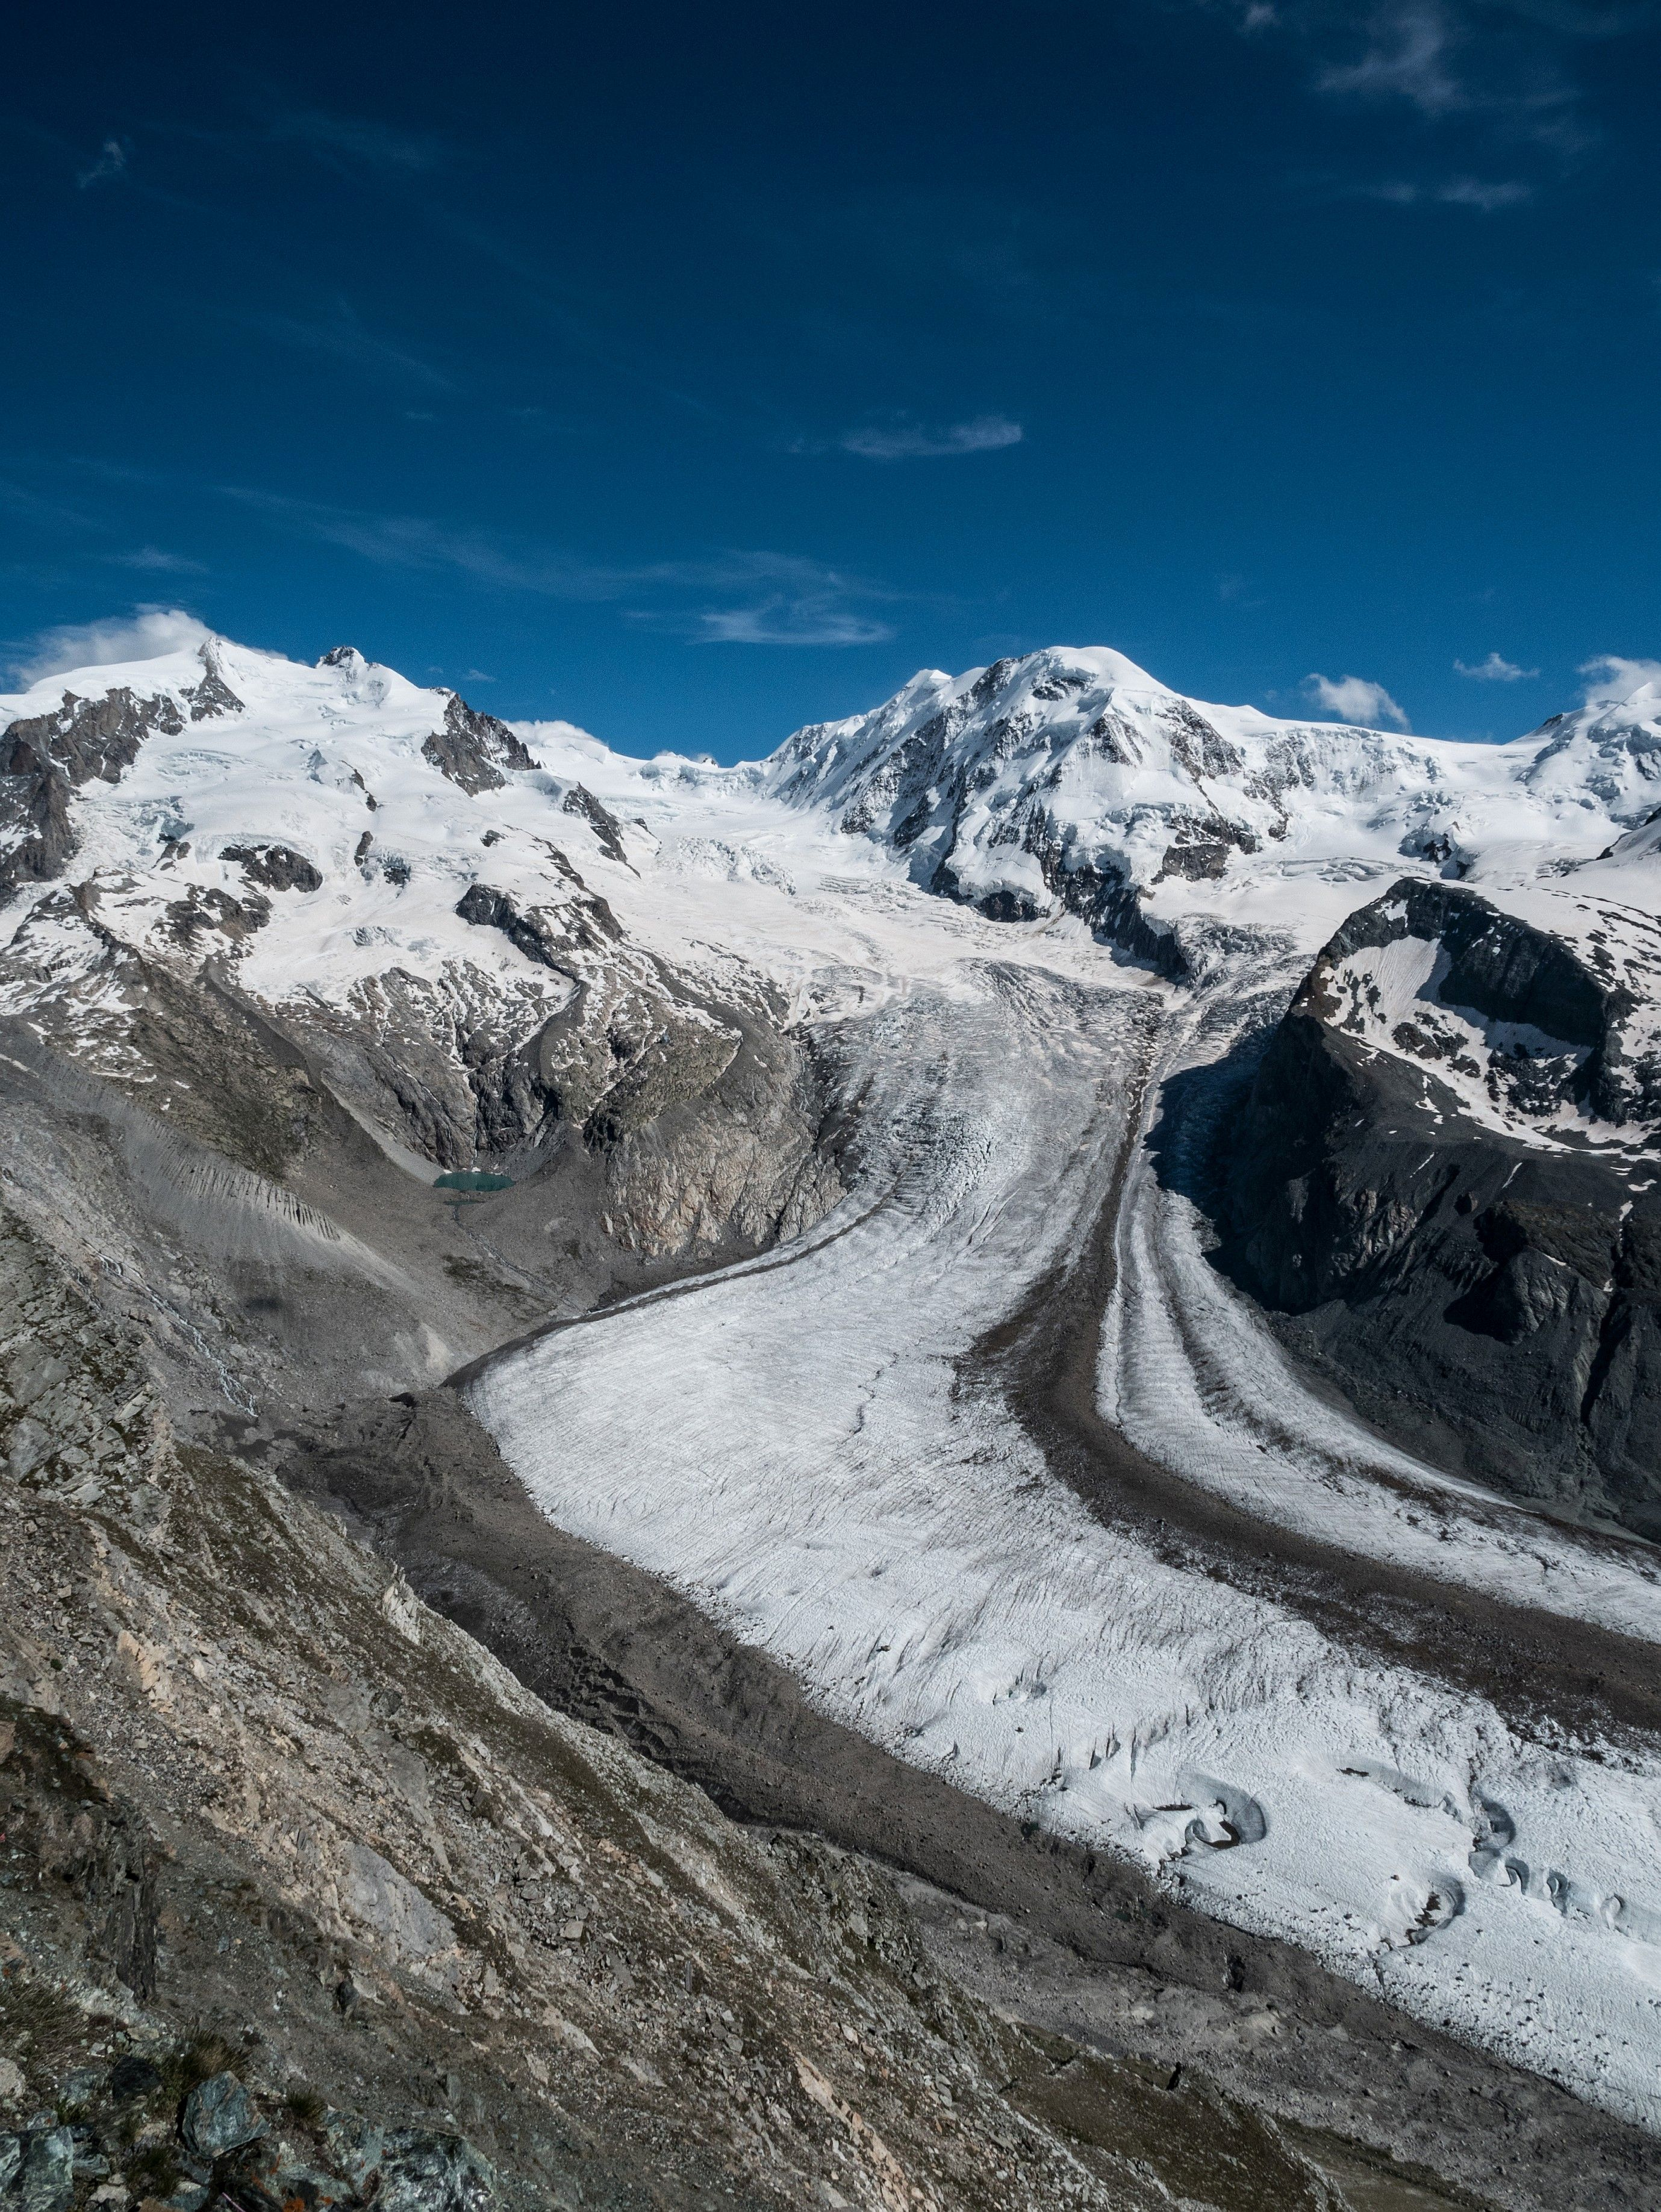
\includegraphics[width=1\linewidth]{obrazky/glac/ledovec_svyc}
	\caption{Horský ledovec s dobře patrnou střední morénou. V pravém dolním rohu je klikatící se supraglaciální tok.}
	\label{fig:ledovec}
\end{figure}


\subsection{Glaciální transport a akumulace}
%TODO GLaciální transport a akaumulace
\begin{figure}
	\centering
	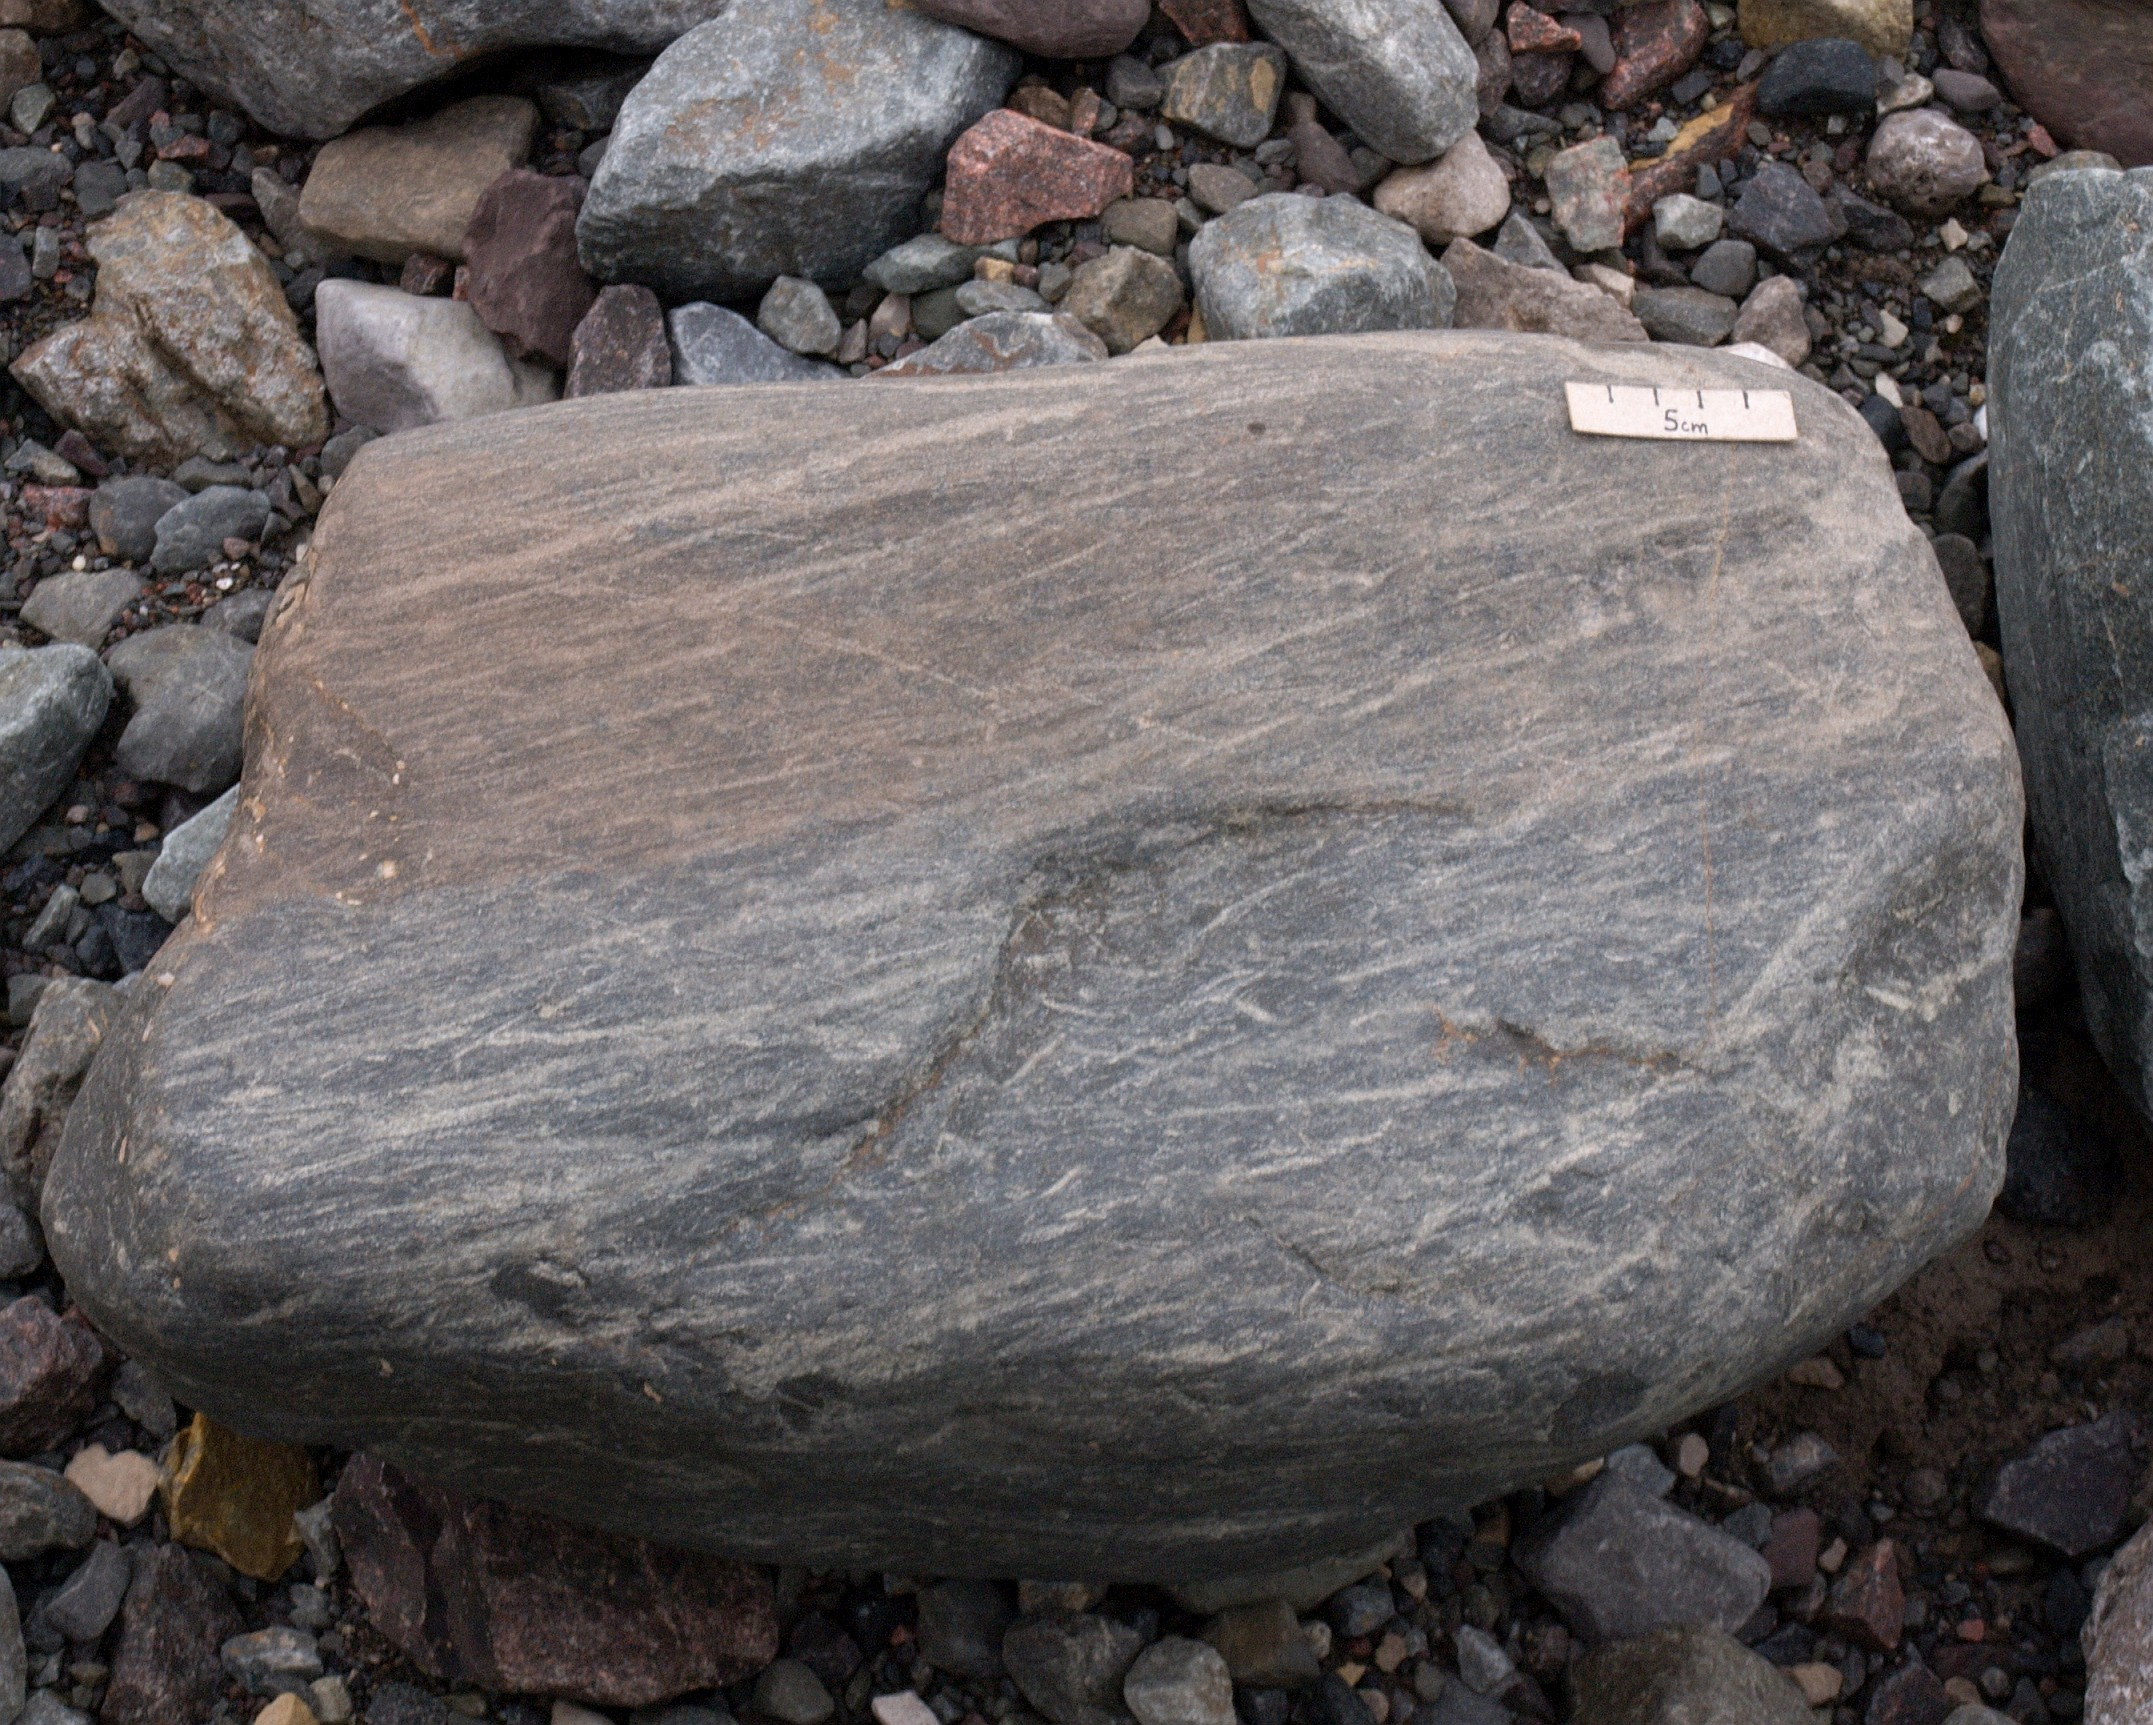
\includegraphics[width=1\linewidth]{obrazky/glac/striace}
	\caption{Striace jsou důkazem subglaciálního transportu (na bázi ledovce).}
	\label{fig:striace}
\end{figure}

\section{Ledovcové tvary}
\subsection{Tvary ledovcové eroze}
Ledovce svou abrazní činností vytvářejí na skalách hladké plochy -- \emph{ledovcové ohlazy}. Materiál transportovaný na bázi ledovce obrušuje a škrábe podloží. Tímto obrušováním vznikají rýhy, které nazýváme \emph{ledovcové striace}. 

Výstupy skalního podloží ledovec přemodelovává v \emph{oblík}, což jsou v podélném profilu asymetrické pahorky. Svah ukloněný proti pohybu ledovce je mírný, hladký a nese stopy po obrušování (striace). Svah po směru pohybu je naopak strmý a s různými výstupky, které vznikly vytrháváním kusů hornin. 

\begin{figure}
	\centering
	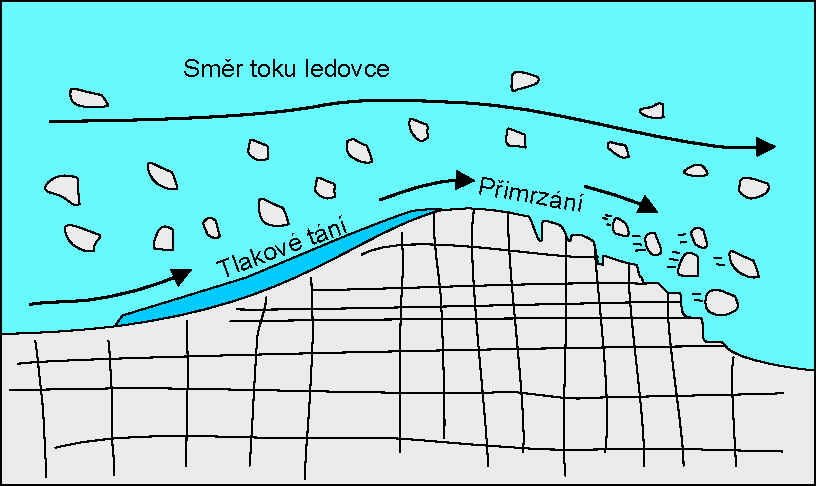
\includegraphics[width=1\linewidth]{obrazky/glac/oblik}
	\caption{Oblík}
	\label{fig:oblik}
\end{figure}

V uzávěrách údolí, pramenných oblastech říčních údolí vznikají ledovcovou erozí \emph{kary} (\textit{cirque}). Tvar karu by se dal připodobnit křeslu. Vysoké a strmé stěny karu navazují na prohloubené konkávní dno karu. Od údolí je kar oddělen karovým stupněm.

Ústupem zadních stěn karů z více stran vznikají ostré horské \emph{štíty} taktéž známé jako \emph{karlingy}, \emph{\^{a}rety} nebo \emph{(matter)horn} podle typického horského štítu Matterhorn (Obr. \ref{fig:matterhorn}) ve Švýcarských alpách.

\begin{figure}
	\centering
	\includegraphics[width=1\linewidth]{obrazky/glac/matterhorn}
	\caption{Matterhorn (Autor: Davide Notti (distributed via imaggeo.egu.eu, CC BY 3.0))}
	\label{fig:matterhorn}
\end{figure}

\emph{Trog} je ledovcové údolí. Jeho příčný profil má tvar písmene \enquote{U}. V podélném profilu trogů jsou patrné stupně, které mohou například souviset se strukturní predispozicí či změnou litologie. Ledovcová údolí mající dno pod hladinou moře se nazývají \emph{fjordy}.

\emph{Visutá údolí} jsou boční údolí trogu. Menší ledovce nemají takový erozivní účinek aby údolí prohloubily na úroveň hlavního trogu. Na těchto stupních pak po odlednění bývají vodopády.

\begin{figure*}
	\centering
	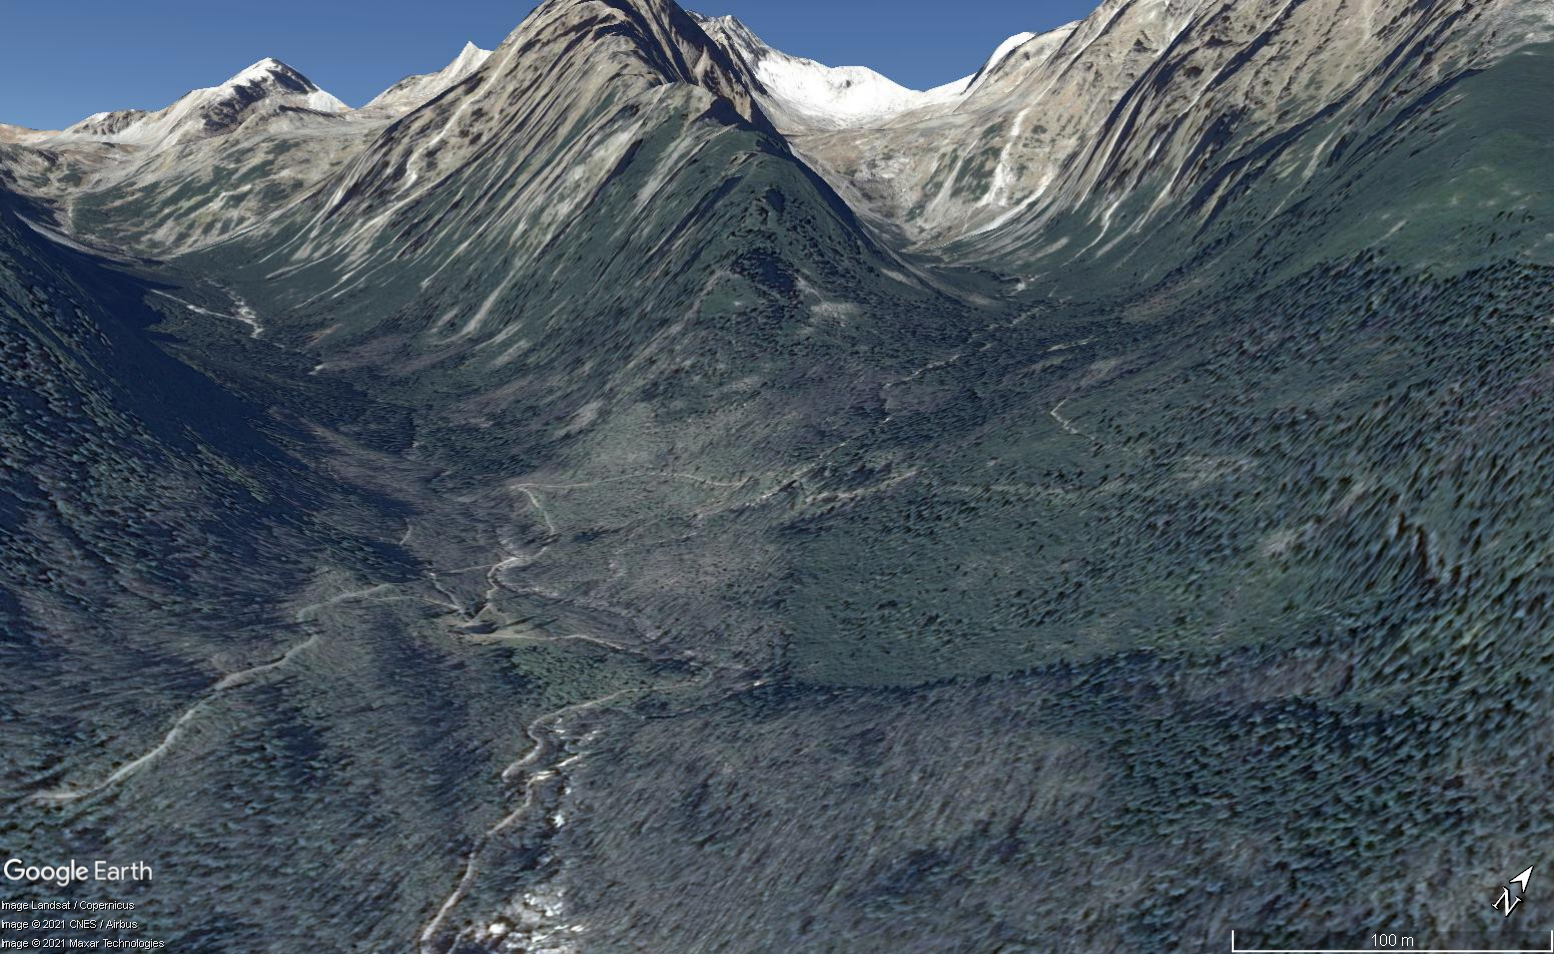
\includegraphics[width=1\linewidth]{obrazky/glac/studena}
	\caption{Typické trogy. Pohled do Velké a Malé Studené doliny ve Vysokých Tatrách. Malá Studená Dolina je příklad visutého údolí (Zdroj: Google Earth)}
	\label{fig:studena}
\end{figure*}

\emph{Nunataky} jsou izolované skály ze všech stran obklopené ledovcem.

\subsection{Tvary ledovcové akumulace}
Glaciální sediment se nazývá \emph{till}. Je tvořen nevytříděným materiál (obsahuje různé frakce). Till obshuje různě opracovaný materiál -- jak ostrohranné, tak i zaoblené klasty. Na klastech jsou patrné ohlazy a \emph{striace}. Till je nevrstevnatý a litologicky heterogenní.

Akumulační formy tvořené tillem se označují jako \emph{morény}. Morény jsou důležitým indikátorem dynamiky ledovce, jeho maximálního rozsahu apod. Rozlišujeme několik základních druhů morén. \emph{Čelní morény} jsou valy, které vznikají před čelem ledovce. Omezují nejzazší místo, kam se ledovec dostal. \emph{Boční morény} jsou akumulace po bocích ledovce. Při spojení dvou ledovců dochází i ke splynutí jejich bočních morén, vzniká tak \emph{střední moréna}. \emph{Ústupové morény} jsou drobnější morény mezi čelní morénou a zbytkem ledovce případně karem. Vyznačují místa, kde došlo ke krátkodobé stabilizaci ustupujícího ledovce. \emph{Svrchní moréna} pokrývá ledovec. Malá vrstva svrchní morény snižuje albedo a může způsobit intenzivnější tání ledovce. Pokud je ale svrchní moréna mocnější, tak může naopak působit jako izolant. Materiál v těle ledovce označujeme jako \emph{vnitřní morénu}. V podloží ledovce se nachází \emph{spodní moréna}.

\emph{Drumlin} může na první pohled připomínat oblík. Je tvořen ale sedimenty a jeho podélný profil je opačný. Strmý svah je proti pohybu ledovce a mírný svah po směru pohybu. 
%TODO Drumln obrázek

Táním tzv. mrtvého ledu (ledových čoček) vznikají sníženiny, které mohou být vyplněné vodou. Označují se jako \emph{kotlíkové jámy} a v případně zaplnění vodou \emph{kotlíková jezera} (\textit{kettle lakes}).

\subsection{Fluvioglaciální tvary reliéfu}
\emph{Sandry} jsou ploché výplavové kužely vzniklé rozplavováním čelních morén a glaciálně transportovaných jemných sedimentů. Sandry jsou tedy tvořené zejména písčitým materiálem. 

\emph{Glacifluviální kužely} jsou obdobou sandrů, ale jsou tvořeny štěrkovým materiálem, který je transportován divočícími toky.

\emph{Eskery} (ózy). Jsou protáhnuté valy vytvořené akumulací sedimentů v subglaciálních tocích. Fluvioglaciální materiál je tříděný.

\begin{figure}
	\centering
	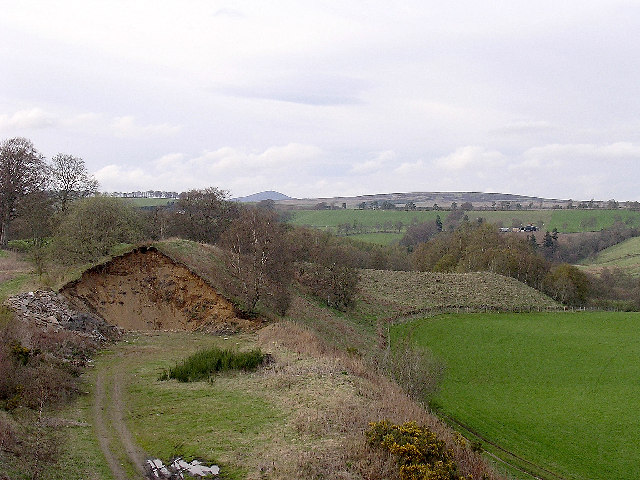
\includegraphics[width=1\linewidth]{obrazky/glac/esker}
	\caption{Částečně odtěžený esker (Autor: Val Vannet / Esker near Bridge of Cally / CC BY-SA 2.0).}
	\label{fig:esker}
\end{figure}

\emph{Kamy} jsou nepravidelné pahorky glacifluviálního materiálu na povrchu spodní morény. Vznikají sesedáním sedimentů supraglaciálních (tekoucích po povrchu ledovce) toků po deglaciaci. V okrajových partiích ledovce, podél údolních svahů se mohou tvořit \emph{kamové terasy}.

\newpage
\onecolumn
\begin{boxotazky}{Kontrolní a klíčové otázky, na které bychom měli znát odpověď}
	\begin{itemize}
		\item Jakým způsobem ledovce nabírají hmotu? 
		\item Co je to tzv. čára rovnováhy a jak její posun ovlivňuje ledovec?
		\item Jaký je rozdíl mezi ledovci, které nejsou ovlivněné reliéfem v podloží a těmi, které naopak ovlivněné jsou?
		\item Jakým způsobem ovlivňuje teplota báze ledovce jeho pohyb a erozní schopnosti?
		\item Jak lze z podoby oblíku a drumlinu poznat směr pohybu ledovce?
		\end{itemize}
\end{boxotazky}

\begin{boxslovnik}{Další klíčové pojmy k zapamatování}
	firn & ablace \\
	čára rovnováhy & ledový proud \\
	šelfový ledovec & kontinentální ledovec \\
	kar & trog \\
	oblík & nunatak \\
	striace & moréna \\
	till & kotlíková jezera \\
	sandr & esker \\
\end{boxslovnik}
\twocolumn